% Generated by code/ch13_twoqubit_id.py -- do not edit by hand.
\definecolor{qocA}{rgb}{0.00,0.45,0.70}
\definecolor{qocB}{rgb}{0.90,0.60,0.00}
\definecolor{qocC}{rgb}{0.00,0.62,0.45}
\definecolor{qocD}{rgb}{0.80,0.40,0.00}
\definecolor{qocE}{rgb}{0.80,0.60,0.70}
\definecolor{qocF}{rgb}{0.35,0.70,0.90}
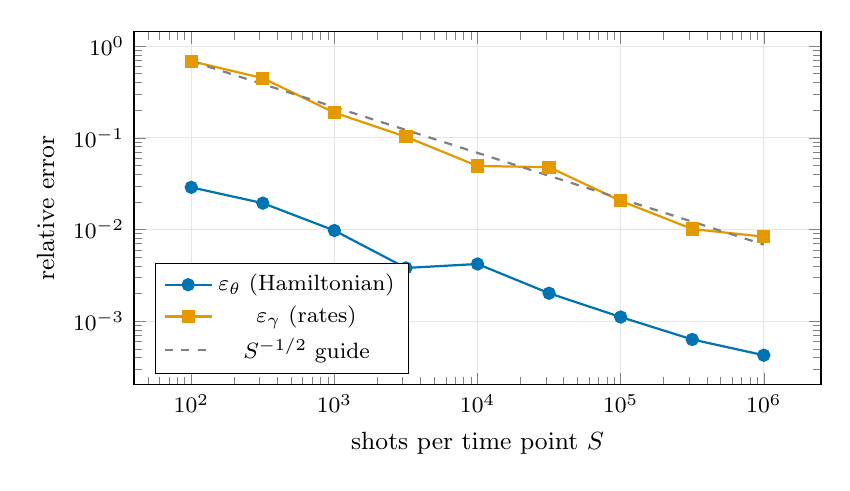
\begin{tikzpicture}[]
\begin{axis}[width=0.85\linewidth, height=0.5\linewidth, xlabel={shots per time point $S$}, ylabel={relative error}, legend pos=south west, legend style={font=\footnotesize}, tick label style={font=\footnotesize}, label style={font=\small}, grid=major, grid style={gray!20}, xmode=log, ymode=log]
\addplot[thick, qocA, mark=*] coordinates {(100,0.028857) (316.23,0.019409) (1000,0.0097599) (3162.3,0.003812) (10000,0.0042107) (31623,0.0020205) (1e+05,0.0011118) (3.1623e+05,0.00063305) (1e+06,0.00042609)};
\addplot[thick, qocB, mark=square*] coordinates {(100,0.68561) (316.23,0.44725) (1000,0.18827) (3162.3,0.10274) (10000,0.049347) (31623,0.047916) (1e+05,0.020569) (3.1623e+05,0.010135) (1e+06,0.0083538)};
\addplot[thick, qocC, dashed, gray] coordinates {(100,0.68561) (316.23,0.38555) (1000,0.21681) (3162.3,0.12192) (10000,0.068561) (31623,0.038555) (1e+05,0.021681) (3.1623e+05,0.012192) (1e+06,0.0068561)};
\legend{$\varepsilon_\theta$ (Hamiltonian), $\varepsilon_\gamma$ (rates), $S^{-1/2}$ guide}
\end{axis}
\end{tikzpicture}
